\documentclass{journal}
\usepackage{blindtext}
\usepackage[a4paper, total={6in,8in}]{geometry}
\usepackage{graphicx} % Required for inserting images
\usepackage{float} % for cramming graphs into place
\usepackage{times} % times new roman font

\usepackage{listings}
\usepackage{xcolor}

\graphicspath{./}

\usepackage[utf8]{inputenc}
\usepackage[english]{babel}
\usepackage[backend=biber,style=chem-acs,biblabel=dot,articletitle=true]{biblatex}
\usepackage{csquotes}
\usepackage{url}
\addbibresource{./references.bib} %TODO: prepare .bib file.

%% Define a new 'leo' style for the package that will use a smaller font.
\makeatletter
\def\url@leostyle{%
  \@ifundefined{selectfont}{\def\UrlFont{\sf}}{\def\UrlFont{\small}}}
\makeatother
%% Now actually use the newly defined style.
\urlstyle{leo}


\definecolor{codegreen}{rgb}{0,0.6,0}
\definecolor{codegray}{rgb}{0.5,0.5,0.5}
\definecolor{codepurple}{rgb}{0.58,0,0.82}
\definecolor{backcolour}{rgb}{0.95,0.95,0.92}

\lstdefinestyle{mystyle}{
    backgroundcolor=\color{backcolour},   
    commentstyle=\color{codegreen},
    keywordstyle=\color{magenta},
    numberstyle=\tiny\color{codegray},
    stringstyle=\color{codepurple},
    basicstyle=\ttfamily\footnotesize,
    breakatwhitespace=false,         
    breaklines=true,                 
    captionpos=b,                    
    keepspaces=true,                 
    numbers=left,                    
    numbersep=5pt,                  
    showspaces=false,                
    showstringspaces=false,
    showtabs=false,                  
    tabsize=2
}

\lstset{style=mystyle}



\newcounter{equationCounter}
\newcounter{figureCounter}
\newcounter{tableCounter}


\usepackage[]{fancyhdr}
\title{Photoelectric Python}
\author{Gage Bayliss}
\date{\today}


\begin{document}

\fancyhead[L]{\@title}
\fancyfoot[L]{\@author}

\makeatletter
\begin{titlepage}

The title is \@title\\
It was written by \@author\space on \@date

\end{titlepage}
\makeatother

\section*{Photoelectric Effect Python Experiment}


\paragraph{}
Go to \url{https://applets.kcvs.ca/photoelectricEffect/PhotoElectric.html#} to start your simulation experiment to collect data to use in your Python code. In the options menu on the upper left-hand corner, select a metal to analyze.  You can choose from Cs, Ca, K, or Na. Adjust the wavelength to 200 nm.  Record the frequency.  Adjust the voltage by 0.25 and click record the data point.  You can stop recording data once you have reached 5 V, click show data and download the CSV.  Save the CSV file according to the name of the metal you are analyzing and the wavelength.  Use an underscore instead of a space to save the file (Example Cs\_200nm.csv). Go to the upper left-hand corner under options and clear the data.  Start the process again at 250, 300, 350, 400, 450, and 500 nm.    Put these files in your Python folder in the Photoelectric effect experiment on your desktop.

\paragraph{}
First, import the necessary libraries to work with your data.
\begin{lstlisting}[language=python]
import pandas as pd
import numpy as np
import matplotlib.pyplot as plt
import os #for manipulating files
import re #regular expressions for manipulating text
\end{lstlisting}

\section*{Part 1}
\paragraph{}
First, we will write our plotting function for this data set. It will accept a dataframe object with our data points, the labels of the x and y columns, a title to display, the coefficients of the trendline to plot, and the filename to save a png image to. 

\begin{lstlisting}[language=python]
def plot_data(dataframe,x_column,y_column,title,trendline_coeffs=None,output_file=None):
    x = dataframe[x_column]
    y = dataframe[y_column]

    plt.scatter(x,y, label = 'Data Points', color='blue')

    plt.xlabel(x_column)
    plt.ylabel(y_column)
    plt.title(title)

    if trendline_coeffs is not None:
        poly_coeff = trendline_coeffs
        poly_degree = len(trendline_coeffs) -1
        poly = np.poly1d(poly_coeff)
        x_fit = np.linspace(x.min(),x.max(), 500)
        y_fit = poly(x_fit)
    
        plt.plot(x_fit, y_fit, label=f'Polynomial Fit (Degree {poly_degree})',color='red')
        
        equation_text = "$y = " + " + ".join([f"{coef:.3e}x^{poly_degree - i}" if i != poly_degree else f"{round(coef, 3)}"
                                              for i, coef in enumerate(poly_coeff)]) + "$"
        plt.text(0.2,0.8, equation_text, transform=plt.gca().transAxes, fontsize=8,
                 verticalalignment='bottom', horizontalalignment='left')
        plt.legend()

    if output_file:
        plt.savefig(output_file,format='png',dpi=300, bbox_inches='tight')
        
    plt.show()
\end{lstlisting}

\paragraph{}
Now, we will use this newly created plot function to display the data we collected. Load your data from your csv files into a pd.DataFrame object. 

\begin{lstlisting}[language=python]
file_path = 'Ca_200nm.csv'
data = pd.read_csv(file_path)
\end{lstlisting}
\paragraph{}
Define the x column and y column and format your title. 
\begin{lstlisting}[language=python]
xcol = 'Voltage (V)'
ycol = 'Current (pA)'
title = f'{ycol} vs {xcol} for Ca Metal at 200nm'
\end{lstlisting}
\paragraph{}
Finally, we are ready to call our plot function.
\begin{lstlisting}[language=python]
plot_data(data,xcol,ycol,title,output_file='Ca_200nm.png')
\end{lstlisting}
\paragraph{}
Your output should look something like this. If it doesn't, you should get a TA to help before proceeding.
    \begin{figure}[H]
        \centering
        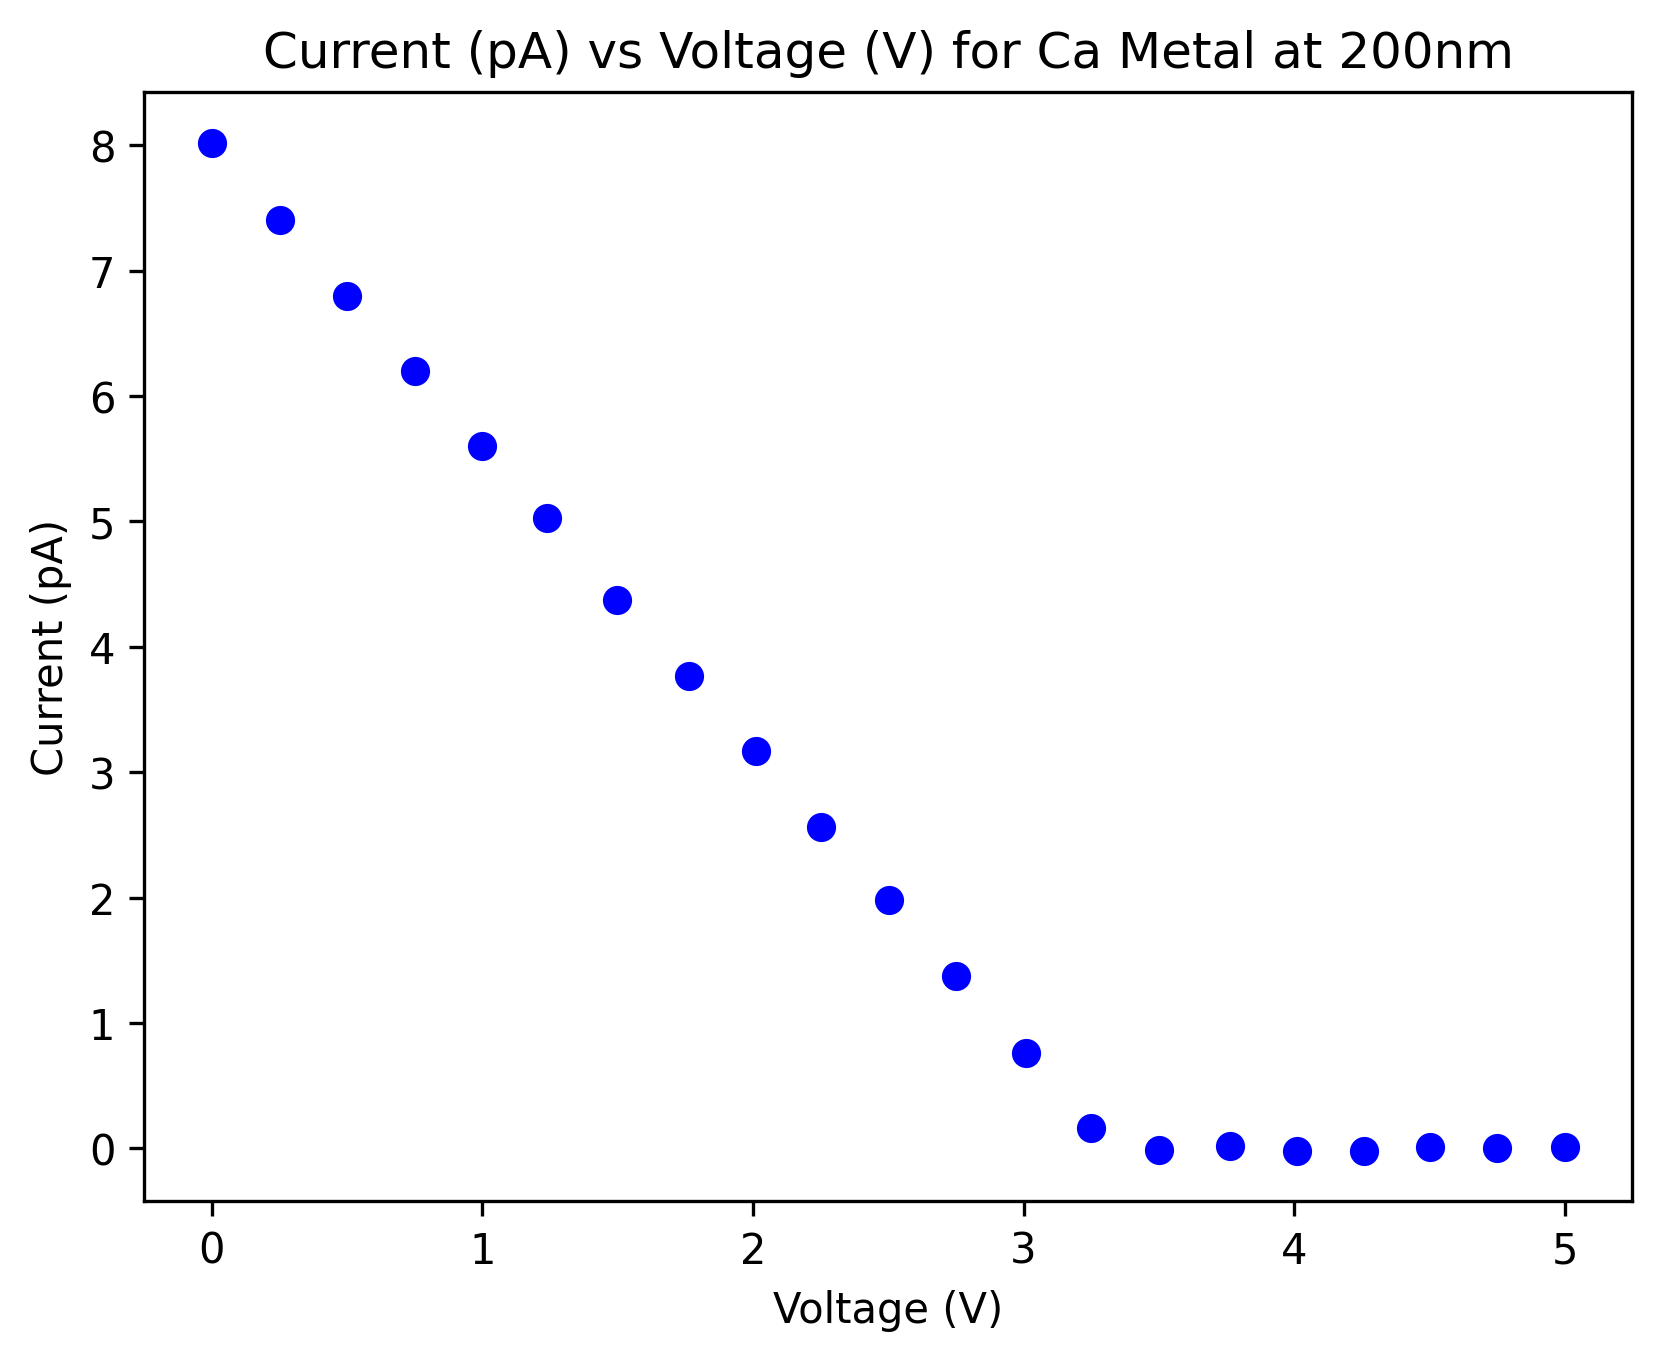
\includegraphics[width=0.5\textwidth]{./Ca_200nm.png}
    \end{figure}

\section*{Part 2}
\paragraph{}
Now we will perform a polynomial fit on our data, and plot the best-fit curve. First, we will use NumPy's polyfit function to obtain a tuple of polynomial coefficients.
\begin{lstlisting}[language=python]
poly_degree = 4
poly_coeff = np.polyfit(data[xcol],data[ycol],poly_degree)
\end{lstlisting}
\paragraph{}
Plotting our data with the fit is as simple as re-using the line of code we used to plot it without, except that we add the polynomial coefficients as a parameter.
\begin{lstlisting}[language=python]
plot_data(data,xcol,ycol,title,poly_coeff,output_file='Ca_200nm.png')
\end{lstlisting}
\paragraph{}
Your output should look something like this. Again, if it doesn't, get a TA to help.
    \begin{figure}[H]
        \centering
        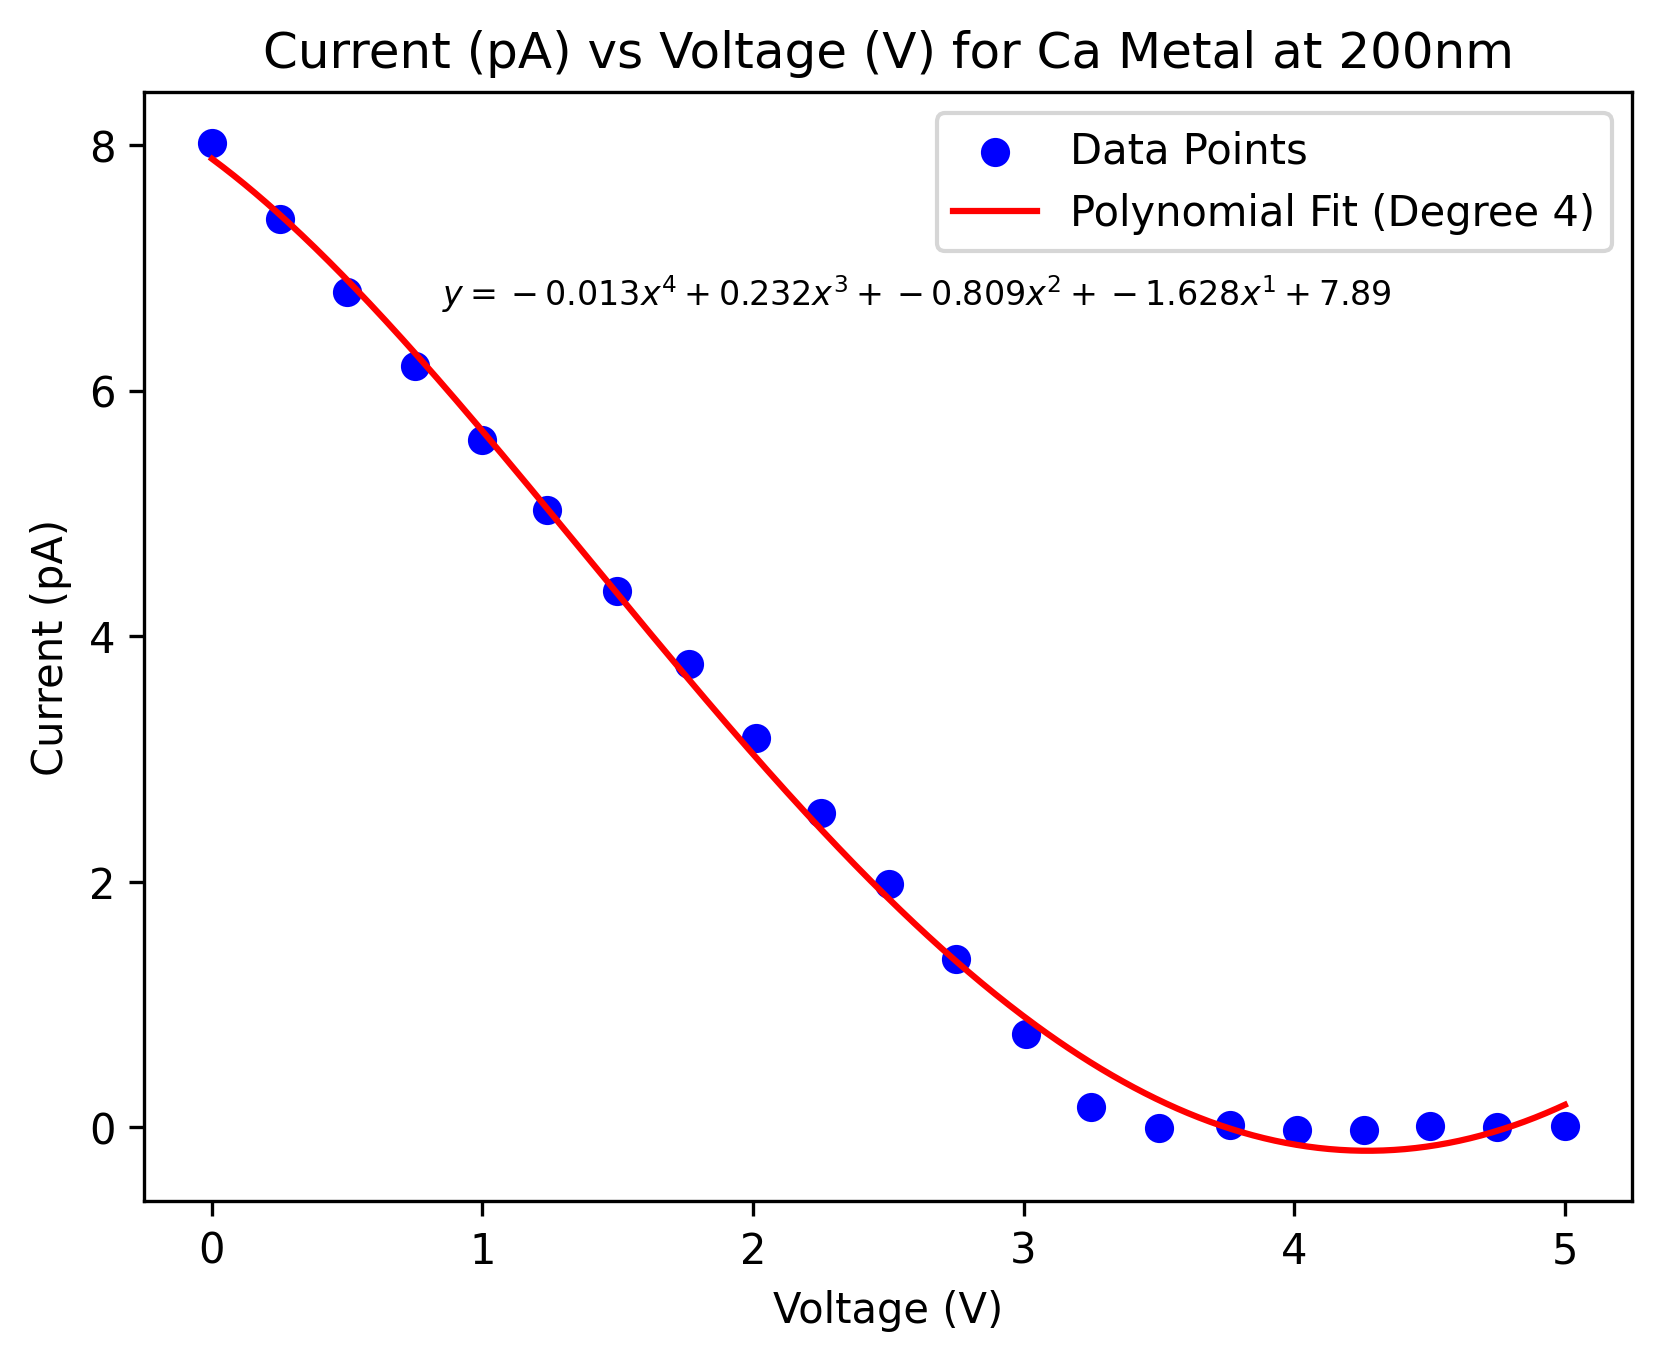
\includegraphics[width=0.5\textwidth]{./Ca_200nm_polyfit.png}
    \end{figure}

\paragraph{}
Calculate the y intercept and smallest positive root of the polynomial fit. We will use the smallest positive root as the cutoff voltage, $V_0$.
\begin{lstlisting}[language=python]
def find_root_and_yint(data,x_column,y_column,poly_degree=2,interval=[0,np.inf]):
    x = data[x_column]
    y = data[y_column]
    poly_coeff = np.polyfit(x,y,poly_degree)
    root = min([float(root) for root in np.roots(poly_coeff) if interval[0] < root and root < interval[1]])
    yint = float(poly_coeff[-1])
    return root,yint
\end{lstlisting}
\paragraph{}
Here is an example of using this function to obtain the cutoff voltage for our data set:
\begin{lstlisting}[language=python]
root_yint = find_root_and_yint(data,'Voltage (V)', 'Current (pA)', poly_degree)
poly_V0 = root_yint[0]
print(f"for degree {poly_degree} fit : root: {root_yint[0]:.3f} ; y-intercept: {root_yint[1]:.3f}")
\end{lstlisting}
\paragraph{}
In your answer to Part 2, show your code, the plot with polynomial fit, and the calculated y intercept and $V_0$.

\break{}
\section*{Part 3}
\paragraph{}
Now, we will repeat all of this using a linear regression. Because there are many zero data points which we do not want, we will need to write a function that will truncate our data so that it does not include these.
\begin{lstlisting}[language=python]
def truncate_data(dataframe,xcol,ycol,y_threshold):
    '''
    returns a dataframe including only the first value
    lower than or equal to y_threshold
    '''
    for index, y_value in enumerate(dataframe[ycol]):
        if y_value <= y_threshold:
            #return dataframe only up to and including this value
            return dataframe.iloc[0:index + 1]
    #nothing was below threshold
    return dataframe
\end{lstlisting}
\paragraph{}
Now, plot your truncated data. It should look something like this; if it doesn't, you will once more need to bother your TA.
    \begin{figure}[H]
        \centering
        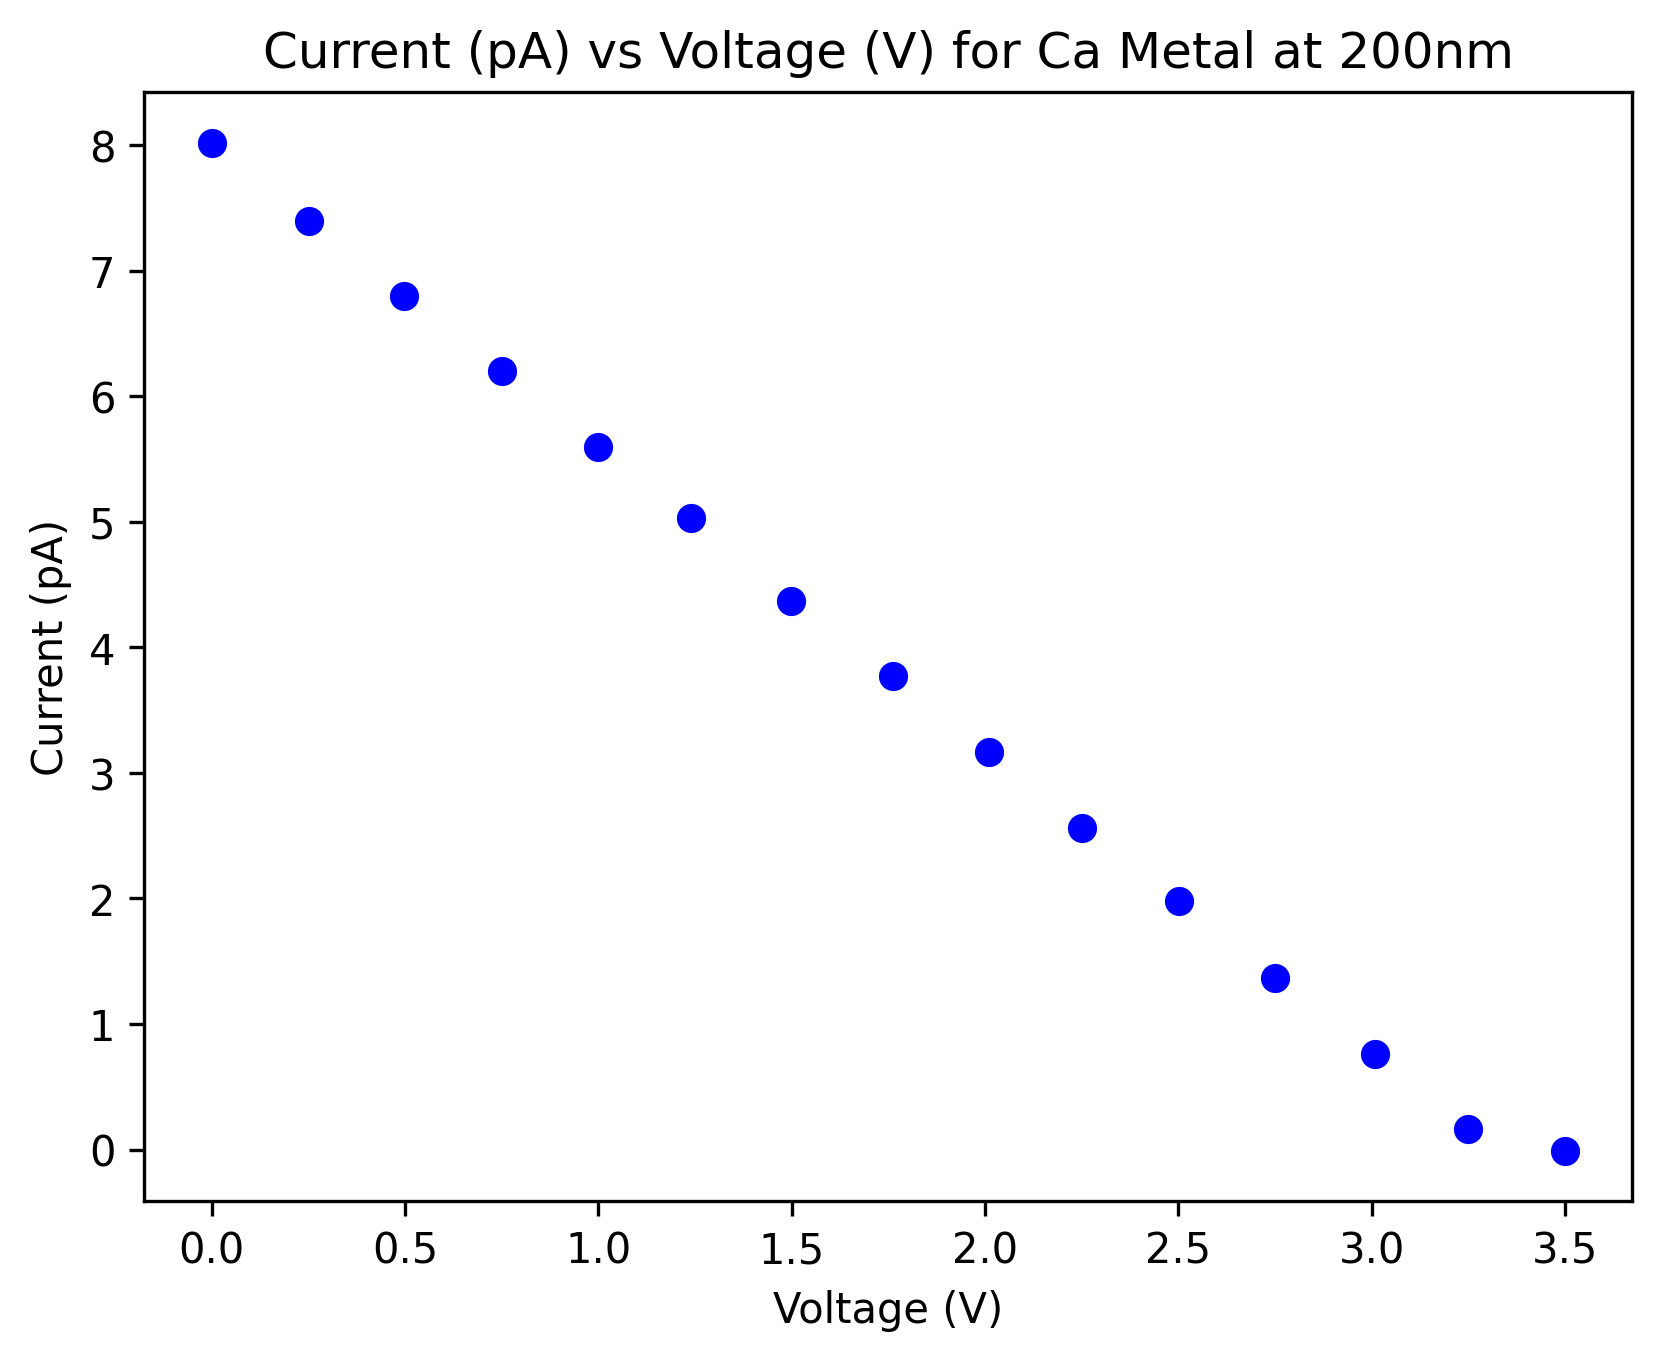
\includegraphics[width=0.5\textwidth]{./Ca_200nm_trunc.png}
    \end{figure}

\paragraph{}
Once we have prepared our truncated graph, repeating this procedure with a linear regression is as easy as re-using all our old functions in the same order, with the only changes being the filename and setting poly\_degree = 1.
\begin{lstlisting}[language=python]
#This is all that changes!
poly_degree = 1
filename = 'Ca_200nm_trunc_linear'
#all this is the same!
poly_coeff = np.polyfit(data[xcol],data[ycol],poly_degree)
plot_data(data,xcol,ycol,title,poly_coeff,output_file=filename)
root_yint = find_root_and_yint(data,'Voltage (V)', 'Current (pA)', poly_degree)
lin_V0 = root_yint[0] #I lied, this line is different
print(f"for degree {poly_degree} fit : root: {root_yint[0]:.3f} ; y-intercept: {root_yint[1]:.3f}")       
\end{lstlisting}
\paragraph{}
For your answer to part 3, include the code you used for this section, the graphical output, and the calculated root and y-intercept.



\section*{Part 4}
\paragraph{}
Now, we are at the good stuff. We will calculate the work function of the metal, using the stopping potential calculated by finding the root of our regression. Write a function to calculate $\phi$ for your metal, using the formula $\phi = h\nu - e V_0$.
\paragraph{}
We will define the physical constants we will continually use:
\begin{lstlisting}[language=python]
c = 3e8
h = 6.626e-34
e = 1.602e-19
\end{lstlisting}
\begin{lstlisting}[language=python]
#this one's on you... it's just arithmetic!
def calculate_phi(V_0,wavelength_nm):
    #your function body goes here
    return phi
\end{lstlisting}
\paragraph{}
Next, calculate phi for the polynomial fit, and for the linear fit. Are they significantly different?
\begin{lstlisting}[language=python]
phi_poly = calculate_phi(poly_V0,200)
phi_lin = calculate_phi(lin_V0,200)    
print(f'Phi_poly : {phi_poly}')
print(f'Phi_linear : ' + str(phi_lin))
\end{lstlisting}
\paragraph{}
In your answer to Part 4, show your code and the output you obtained, as well as any commentary on the differences between these values.

\section*{Part 5}
Here, we will calculate the cutoff frequency (and wavelength) for our metal using the work function obtained in Part 4. Remember, $V_0 = (\frac{h}{e}\nu) - (\frac{\phi}{e}) = 0$.
\begin{lstlisting}[language=python]
def calculate_cutoff_nu_lambda(phi):
    #your logic goes here
    return nu_cutoff_Hz,lambda_cutoff_nm
\end{lstlisting}
\paragraph{}
Now, use this to obtain values of cutoff frequency for each regression technique.

\begin{lstlisting}[language=python]
lin_nu_lambda = calculate_cutoff_nu_lambda(phi_lin)
nu_cutoff_lin = lin_nu_lambda[0]
print(f'Cutoff Frequency (Hz) (degree 1): {nu_cutoff_lin:.0f}')
lambda_cutoff_lin = lin_nu_lambda[1]
print(f'Cutoff Wavelength (nm) (degree 1): {lambda_cutoff_lin:.0f}')

poly_nu_lambda = calculate_cutoff_nu_lambda(phi_poly)
nu_cutoff_poly = poly_nu_lambda[0]
print(f'Cutoff Frequency (Hz) (degree 4): {nu_cutoff_poly:.0f}')
lambda_cutoff_poly = poly_nu_lambda[1]
print(f'Cutoff Wavelength (nm) (degree 4): {lambda_cutoff_poly:.0f}')
\end{lstlisting}

\paragraph{}
For this section, show your calculate\_cutoff\_nu\_lambda function and the output you obtain.

\section*{Part 6}
\paragraph{}
Now, we will bring it all together. We will create a function using every function we have created so far, which accepts a dataframe, an x column label and y column label, the wavelength in nm, and the polynomial degree, and returns all the derivable values in a Python dict object.

\begin{lstlisting}[language=python]
def process_data(dataframe,xcol,ycol,lambda_nm,poly_degree):
    data = truncate_data(dataframe,xcol,ycol,0.01)
    data_dict = {}

    poly_coeff = np.polyfit(data[xcol],data[ycol],poly_degree)   
    root_yint = find_root_and_yint(data,xcol,ycol, poly_degree)
    V0 = root_yint[0]
    phi = calculate_phi(V0,200)
    nu_lambda = calculate_cutoff_nu_lambda(phi)
    cutoff_nu_Hz = nu_lambda[0]
    cutoff_lambda_nm = nu_lambda[1]

    data_dict['Wavelength(nm)'] = lambda_nm
    data_dict['Frequency(Hz)'] = c / (lambda_nm * 1e-9)
    data_dict['Stopping Potential(V)'] = V0
    data_dict['Work function(J)'] = phi
    data_dict['Cut-off Frequency(Hz)'] = cutoff_nu_Hz
    data_dict['Cut-off Wavelength(nm)'] = cutoff_lambda_nm

    return data_dict
\end{lstlisting}
\paragraph{}
Run this function on your data. Show the output you obtain.
\begin{lstlisting}[language=python]
data_dict= process_data(data,xcol,ycol,200,1)
print(data_dict)
\end{lstlisting}

\section*{Part 7}
\paragraph{}
In this section, we will use this function to read all of the data we collected into a table. You may see a pattern here- once you define a procedure in python, you can scale up by doing it many, many times. Compare this to your experience with excel, which involves all too much manual labor!
\paragraph{}
First, define a method to read all of the files in the directory, and return a dict mapping wavelengths to dataframes.
\begin{lstlisting}[language=python]
def read_files():
    filenames = os.listdir('./') #'./' is the current directory
    csv_files = [file for file in filenames if file.endswith('.csv')]
    data = {}
    for filename in csv_files:
        wavelength_nm = re.search('\d+',filename).group(0)
        data[wavelength_nm] = pd.read_csv(filename)
    return data
\end{lstlisting}


\paragraph{}
Plot all of these data sets to ensure that everything works:
\begin{lstlisting}[language=python]
file_data = read_files()
for _data in file_data:
    trunc_data = truncate_data(file_data[_data],xcol,ycol,0.0)
    plot_data(trunc_data,xcol,ycol,_data)
\end{lstlisting}
\paragraph{}
Now, we will define a function that allows us to process all of our data at once- we bring it all together here.
\begin{lstlisting}[language=python]
def create_table(table_data,poly_degree):
    table = pd.DataFrame({'Wavelength(nm)':[],
                   'Frequency(Hz)':[],
                   'Work Function(J)':[],
                   'Stopping Potential(V)':[],
                   'Cut-off Frequency(Hz)':[],
                   'Cut-off Wavelength(nm)':[]})
    for wavelength in table_data:
        derived_values = process_data(table_data[wavelength],xcol,ycol,wavelength,poly_degree)
        derived_values = {key : [value] for key,value in derived_values.items()}
        row = pd.DataFrame(derived_values)
        numeric_values = pd.to_numeric(row.values.flatten(), errors='coerce')
        if not np.isnan(numeric_values).any():
            table = pd.concat([table,row])
    return table
\end{lstlisting}
\paragraph{}
For your answer to this section, display the table generated by the last function by simply executing a line with only the variable containing it. The output should look something like this:
\begin{figure}[H]
    \centering
    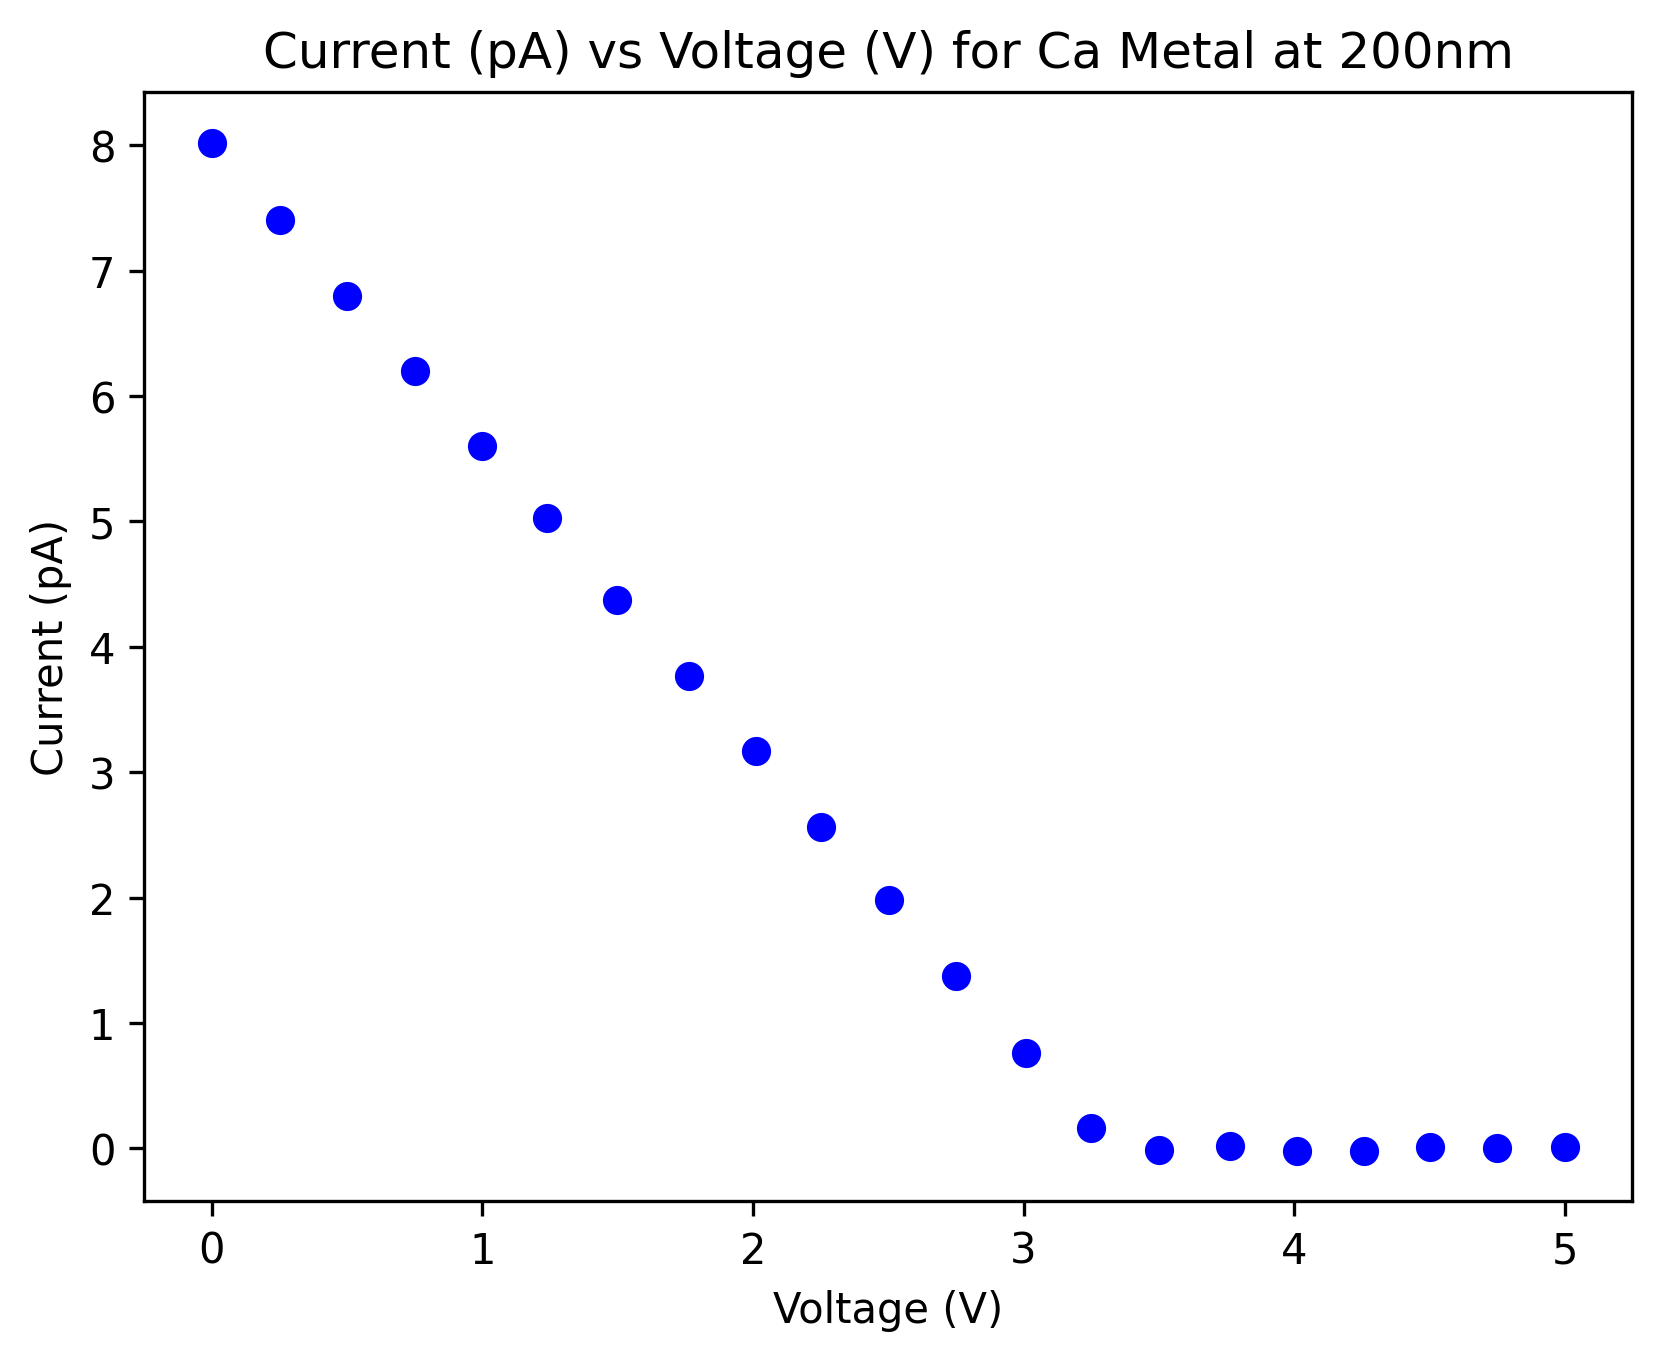
\includegraphics[width=0.5\textwidth]{./Ca_200nm.png}
\end{figure}
\paragraph{}
Include screenshots of your linear and polynomial fit DataFrames in this manner.

\section*{Part 8}
In this section, we will plot this tabulated data to obtain Planck's constant. This will be rather simple; we need only re-use the functions we already have for obtaining coefficients and plotting.

\begin{lstlisting}[language=python]
new_xcol = 'Frequency(Hz)'
new_ycol = 'Stopping Potential(V)' 
title = f'{new_ycol} vs {new_xcol}'
lin_coeff = np.polyfit(table_lin[new_xcol],table_lin[new_ycol],1)
lin_coeff
plot_data(table_lin,new_xcol,new_ycol,'Frequency vs. Stopping Potential',lin_coeff,output_file='PlanckRegression.png')

lin_coeff_poly = np.polyfit(table_poly[new_xcol],table_poly[new_ycol],1)
plot_data(table_poly,new_xcol,new_ycol,'Frequency vs. Stopping Potential',lin_coeff_poly,output_file='PlanckRegression.png')
\end{lstlisting}
\paragraph{}
Find the calculated Planck's constant from the linear coefficients obtained by regression. Compare this to literature values.
\paragraph{}
For your answer to this part, include plots of frequency vs. stopping potential for the tables obtained by both linear and polynomial fits. Print the value of Planck's constant obtained for each, and calculate percent error for each.

\section*{Concluding Questions}
\paragraph{}
Which method of fitting was better? Why do you think this is?
\paragraph{}
How does using Python to process data compare to using tools like Excel?
\paragraph{}
How did we transform our raw data into the data we needed? How could we articulate what we did as a generally applicable problem solving process?
\end{document}

